% =================================================================================================
% File:			client_tier/view.tex
% Description:	Defiinisce la sezione relativa al front-end dell'applicazione
% Created:		2015-04-07
% Author:		Tesser Paolo
% Email:		tesser.paolo@mashup-unipd.it
% =================================================================================================
% Modification History:
% Version		Modifier Date		Change											Author
% 0.0.1 		2015-04-07 			creato scheletro								Tesser Paolo
% =================================================================================================
% 0.0.2			2015-04-07			descrizione delle classi						Carnovalini Filippo
% =================================================================================================
% 0.0.3			2015-04-08			aggiunte classi sulle relazioni					Tesser Paolo
% =================================================================================================
%

% CONTENUTO DEL CAPITOLO

\subsubsection{client::view} % (fold)
\label{ssub:bdsm_app_client_view}
In questa sezione e in tutte quelle inerenti al package \textbf{view}, il termine classe e pagina HTML, saranno sinonimi.
\begin{figure}[htbp]
	\centering
	\centerline{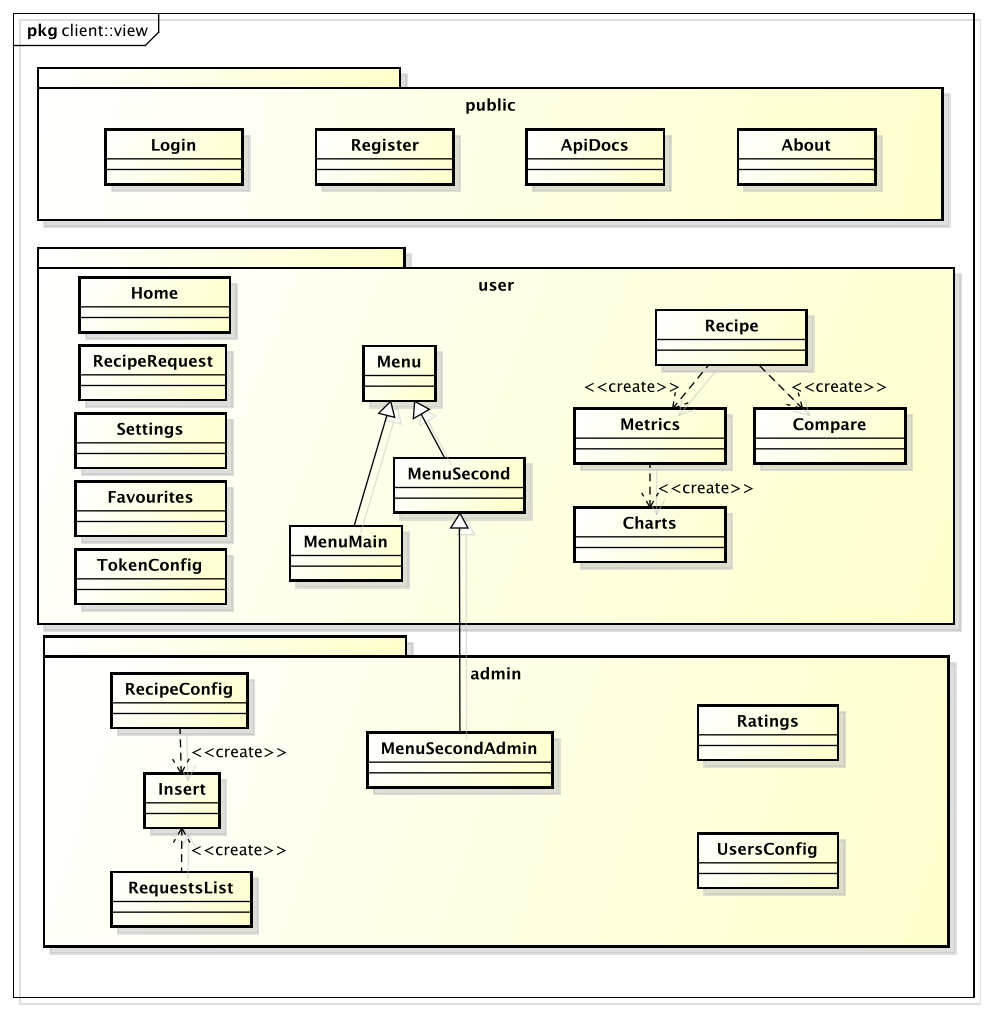
\includegraphics[scale=0.5]{./images/client/client_view.pdf}}
	\caption{Package - client::view}
\end{figure}

\begin{itemize}
	\item \textbf{Descrizione}: è il package che contiene tutte le classi che costituiscono la view del client. Ogni classe è equivalenti a un template di pagina HTML che sarà presentato all'utente, quando richiesto, tramite un sistema di routing. \newline
	All'interno di esso sono presenti altri componenti che separano le pagine HTML offerte, a seconda dei permessi che possiede un utente;
	\item \textbf{Padre}: client
	\item \textbf{Package contenuti}:
		\begin{itemize}
			\item client::view::public
			\item client::view::user
			\item client::view::admin
		\end{itemize}
	\item \textbf{Interazione con altri componenti}:
		\begin{itemize}
			\item client::controller
		\end{itemize}
\end{itemize}
% subsubsection bdsm_app_client_view (end)

\pagebreak

\subsubsection{client::view::public} % (fold)
\label{ssub:bdsm_app_client_view_public}
\begin{figure}[htbp]
	\centering
	\centerline{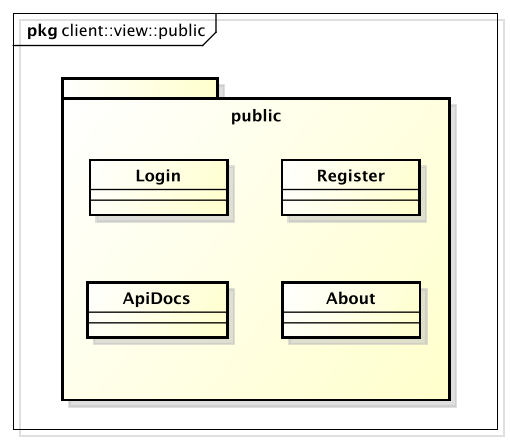
\includegraphics[scale=0.6]{./images/client/client_view_public.pdf}}
	\caption{Package - client::view::public}
\end{figure}

\begin{itemize}
	\item \textbf{Descrizione}: è il package che contiene tutte le pagine HTML che possono essere offerte quando l'utente deve ancora effettuare l'accesso al sistema;
	\item \textbf{Padre}: client::view
	\item \textbf{Interazione con altri componenti}:
		\begin{itemize}
			\item client::controller::public
		\end{itemize}
\end{itemize}

	\paragraph{Classi} % (fold)
		\subparagraph{client::view::public::Login} % (fold)
		\label{subp:bdsm_app_client_view_public_login}
			\begin{itemize}
				\item \textbf{Descrizione}: la classe rappresenta un template HTML per la visualizzazione dell'interfaccia di autenticazione;
				\item \textbf{Utilizzo}: viene utilizzata per generare la pagina HTML di autenticazione;
				\item \textbf{Relazioni con altre classi}:
					\begin{itemize}
						\item client::controller::public::PublicRoute
						\item client::controller::public::LoginCtrl
					\end{itemize}
			\end{itemize}
		% subparagraph bdsm_app_client_view_public_login (end)

		\subparagraph{client::view::public::About} % (fold)
		\label{subp:bdsm_app_client_view_public_about}
			\begin{itemize}
				\item \textbf{Descrizione}: la classe rappresenta un template HTML per la visualizzazione della pagina di informazioni sull'applicazione;
				\item \textbf{Utilizzo}: viene usata per generare la pagina HTML di About;
				\item \textbf{Relazioni con altre classi}:
					\begin{itemize}
						\item client::controller::public::PublicRoute
					\end{itemize}
			\end{itemize}
		% subparagraph bdsm_app_client_view_public_about (end)

		\subparagraph{client::view::public::Register} % (fold)
		\label{subp:bdsm_app_client_view_public_register}
			\begin{itemize}
				\item \textbf{Descrizione}: la classe rappresenta un template HTML per la visualizzazione dell'interfaccia di registrazione al servizio;
				\item \textbf{Utilizzo}: viene utilizzata per generare la pagina HTML di registrazione;
				\item \textbf{Relazioni con altre classi}:
					\begin{itemize}
						\item client::controller::public::PublicRoute
						\item client::controller::public::RegisterCtrl
					\end{itemize}
			\end{itemize}
		% subparagraph bdsm_app_client_view_public_register (end)

		\subparagraph{client::view::public::ApiDocs} % (fold)
		\label{subp:bdsm_app_client_view_public_apidocs}
			\begin{itemize}
				\item \textbf{Descrizione}: la classe rappresenta un template HTML per la visualizzazione della pagina contenente la documentazione dei servizi REST offerti;
				\item \textbf{Utilizzo}: viene utilizzata per generare la pagina HTML contenente la documentazione dei servizi offerti;
				\item \textbf{Relazioni con altre classi}:
					\begin{itemize}
						\item client::controller::public::PublicRoute
						\item client::controller::public::ApiDocsCtrl
					\end{itemize}
			\end{itemize}
		% subparagraph bdsm_app_client_view_public_apidocs (end)

% subsubsection bdsm_app_client_view_public (end)


\subsubsection{client::view::user} % (fold)
\label{ssub:bdsm_app_client_view_user}
\begin{figure}[htbp]
	\centering
	\centerline{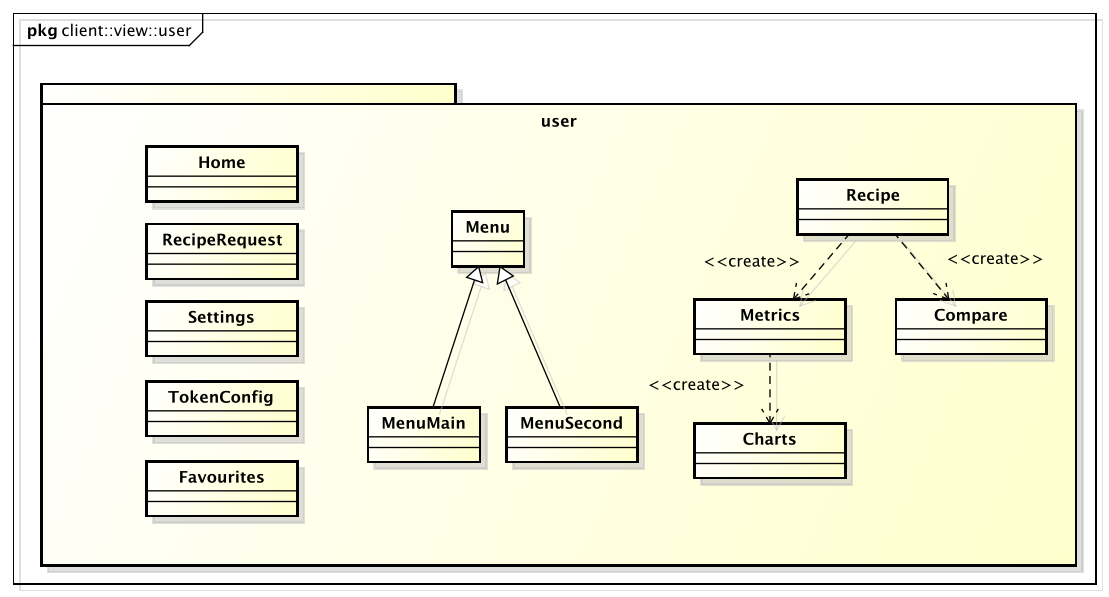
\includegraphics[scale=0.8]{./images/client/client_view_user.pdf}}
	\caption{Package - client::view::user}
\end{figure}

\begin{itemize}
	\item \textbf{Descrizione}: è il package che contiene tutte le pagine HTML che ha a disposizione l'utente che ha effettuato l'accesso al sistema, sia che sia un utente normale sia che sia un amministratore. \newline
	Per semplicità e chiarezza non è stato evidenziato nel grafico il fatto che ogni classe di questo package possiede un'istanza di MenuMain e di MenuSecond.
	\item \textbf{Padre}: client::view
	\item \textbf{Interazione con altri componenti}:
		\begin{itemize}
			\item client::controller::user
		\end{itemize}
\end{itemize}

	\paragraph{Classi} % (fold)
		\subparagraph{client::view::user::Home} % (fold)
		\label{subp:bdsm_app_client_view_user_home}
			\begin{itemize}
				\item \textbf{Descrizione}: la classe rappresenta un template HTML per la visualizzazione dell'interfaccia della home dell'applicazione;
				\item \textbf{Utilizzo}: viene utilizzata per generare la pagina HTML della home;
				\item \textbf{Relazioni con altre classi}:
					\begin{itemize}
						\item client::view::user::MenuMain
						\item client::view::user::MenuSecond
						\item client::controller::public::HomeRoute
						\item client::controller::user::HomeCtrl
					\end{itemize}
			\end{itemize}
		% subparagraph bdsm_app_client_view_user_home (end)

		\subparagraph{client::view::user::Recipe} % (fold)
		\label{subp:bdsm_app_client_view_user_recipe}
			\begin{itemize}
				\item \textbf{Descrizione}: la classe rappresenta un template HTML per la visualizzazione della pagina di visione delle recipe a disposizione;
				\item \textbf{Utilizzo}: viene usata per generare la pagina HTML di visione delle recipe;
				\item \textbf{Relazioni con altre classi}:
					\begin{itemize}
						\item client::view::user::MenuMain
						\item client::view::user::MenuSecond
						\item client::view::user::Metrics
						\item client::view::user::Compare
						\item client::controller::user::RecipeRoute
						\item client::controller::user::RecipeCtrl
					\end{itemize}
			\end{itemize}
		% subparagraph bdsm_app_client_view_user_recipe (end)

		\subparagraph{client::view::user::Metrics} % (fold)
		\label{subp:bdsm_app_client_view_metrics}
			\begin{itemize}
				\item \textbf{Descrizione}: la classe rappresenta un template HTML per la visualizzazione della pagina di visione delle metriche a disposizione per una selezionata recipe;
				\item \textbf{Utilizzo}: viene utilizzata per generare la pagina HTML di visione delle metriche quando viene selezionata una Recipe;
				\item \textbf{Relazioni con altre classi}:
					\begin{itemize}
						\item client::view::user::MenuMain
						\item client::view::user::MenuSecond
						\item client::view::user::Recipe
						\item client::view::user::Charts
						\item client::controller::user::RecipeRoute
						\item client::controller::user::MetricsCtrl
					\end{itemize}
			\end{itemize}
		% subparagraph bdsm_app_client_view_metrics (end)

		\subparagraph{client::view::user::Charts} % (fold)
		\label{subp:bdsm_app_client_view_user_charts}
			\begin{itemize}
				\item \textbf{Descrizione}: la classe rappresenta un template HTML per la visualizzazione della pagina di visione delle view associate ad una metrica selezionata;
				\item \textbf{Utilizzo}: viene usata per generare la pagina HTML di visione delle view quando viene selezionata una metrica;
				\item \textbf{Relazioni con altre classi}:
					\begin{itemize}
						\item client::view::user::MenuMain
						\item client::view::user::MenuSecond
						\item client::view::user::Metrics
						\item client::controller::user::RecipeRoute
						\item client::controller::user::ChartsCtrl
					\end{itemize}
			\end{itemize}
		% subparagraph bdsm_app_client_view_user_charts (end)

		\subparagraph{client::view::user::Compare} % (fold)
		\label{subp:bdsm_app_client_view_user_compare}
			\begin{itemize}
				\item \textbf{Descrizione}: la classe rappresenta un template HTML per la visualizzazione dell'interfaccia di confronto tra diverse metriche di una recipe;
				\item \textbf{Utilizzo}: viene utilizzata per generare la pagina HTML di confronto tra metriche;
				\item \textbf{Relazioni con altre classi}:
					\begin{itemize}
						\item client::view::user::MenuMain
						\item client::view::user::MenuSecond
						\item client::view::user::Recipe
						\item client::controller::user::RecipeRoute
						\item client::controller::user::CompareCtrl
					\end{itemize}
			\end{itemize}
		% subparagraph bdsm_app_client_view_user_compare (end)

		\subparagraph{client::view::user::RecipeRequest} % (fold)
		\label{subp:bdsm_app_client_view_user_reciperequest}
			\begin{itemize}
				\item \textbf{Descrizione}: la classe rappresenta un template HTML per la visualizzazione dell'interfaccia di richiesta di una nuova recipe;
				\item \textbf{Utilizzo}: viene utilizzata per generare la pagina HTML di richiesta di una nuova recipe;
				\item \textbf{Relazioni con altre classi}:
					\begin{itemize}
						\item client::view::user::MenuMain
						\item client::view::user::MenuSecond
						\item client::controller::user::RecipeRequestRoute
						\item client::controller::user::RecipeRequestCtrl
					\end{itemize}
			\end{itemize}
		% subparagraph bdsm_app_client_view_user_reciperequest (end)

		\subparagraph{client::view::user::Favourites} % (fold)
		\label{subp:bdsm_app_client_view_user_favourites}
			\begin{itemize}
				\item \textbf{Descrizione}: la classe rappresenta un template HTML per la visualizzazione della pagina contenente le view preferite;
				\item \textbf{Utilizzo}: viene utilizzata per generare la pagina HTML delle view preferite;
				\item \textbf{Relazioni con altre classi}:
					\begin{itemize}
						\item client::view::user::MenuMain
						\item client::view::user::MenuSecond
						\item client::controller::user::FavouritesRoute
						\item client::controller::user::FavouritesCtrl
					\end{itemize}
			\end{itemize}
		% subparagraph bdsm_app_client_view_user_favourites (end)

		\subparagraph{client::view::user::TokenConfig} % (fold)
		\label{subp:bdsm_app_client_view_user_tokenconfig}
			\begin{itemize}
				\item \textbf{Descrizione}: la classe rappresenta un template HTML per la visualizzazione dell'interfaccia di gestione dei token per l'utilizzo dei servizi REST;
				\item \textbf{Utilizzo}: viene utilizzata per generare la pagina HTML di gestione dei token per i servizi REST;
				\item \textbf{Relazioni con altre classi}:
					\begin{itemize}
						\item client::view::user::MenuMain
						\item client::view::user::MenuSecond
						\item client::controller::user::TokenConfigRoute
						\item client::controller::user::TokenConfigCtrl
					\end{itemize}
			\end{itemize}
		% subparagraph bdsm_app_client_view_user_tokenconfig (end)

		\subparagraph{client::view::user::Settings} % (fold)
		\label{subp:bdsm_app_client_view_user_settings}
			\begin{itemize}
				\item \textbf{Descrizione}: la classe rappresenta un template HTML per la visualizzazione dell'interfaccia di gestione delle opzioni;
				\item \textbf{Utilizzo}: viene utilizzata per generare la pagina HTML delle opzioni;
				\item \textbf{Relazioni con altre classi}:
					\begin{itemize}
						\item client::view::user::MenuMain
						\item client::view::user::MenuSecond
						\item client::controller::user::SettingsRoute
						\item client::controller::user::SettingsCtrl
					\end{itemize}
			\end{itemize}
		% subparagraph bdsm_app_client_view_user_settings (end)

		\subparagraph{client::view::user::Menu} % (fold)
		\label{subp:bdsm_app_client_view_user_menu}
			\begin{itemize}
				\item \textbf{Descrizione}: questa classe astratta rappresenta un template HTML per la creazione di un menù;
				\item \textbf{Utilizzo}: non viene mai istanziata nel sistema, viene ereditata dalla classi che istanziano dei menù;
				\item \textbf{Relazioni con altre classi}:
					\begin{itemize}
						\item client::view::user::MenuMain
						\item client::view::user::MenuSecond
						\item client::controller::user::MenuCtrl
					\end{itemize}
			\end{itemize}
		% subparagraph bdsm_app_client_view_user_menu (end)

		\subparagraph{client::view::user::MenuMain} % (fold)
		\label{subp:bdsm_app_client_view_user_menumain}
			\begin{itemize}
				\item \textbf{Descrizione}: la classe rappresenta un template HTML per la creazione del menù principale;
				\item \textbf{Utilizzo}: viene usata nel generare ogni pagina usata da un utente autenticato per generare il menù principale in essa contenuta;
				\item \textbf{Classi ereditate}:
					\begin{itemize}
						\item client::view::user::Menu
					\end{itemize}
				\item \textbf{Relazioni con altre classi}:
					\begin{itemize}
						\item client::view::user::Menu
						\item client::controller::user::MenuMainCtrl
					\end{itemize}
			\end{itemize}
		% subparagraph bdsm_app_client_view_user_menumain (end)

		\subparagraph{client::view::user::MenuSecond} % (fold)
		\label{subp:bdsm_app_client_view_user_menusecond}
			\begin{itemize}
				\item \textbf{Descrizione}: la classe rappresenta un template HTML per la creazione del menù secondario di un utente non amministratore;
				\item \textbf{Utilizzo}: viene usata nel generare ogni pagina di un utente autenticato non amministratore per generare il menù secondario;
				\item \textbf{Classi ereditate}:
					\begin{itemize}
						\item client::view::user::Menu
					\end{itemize}
				\item \textbf{Relazioni con altre classi}:
					\begin{itemize}
						\item client::view::user::Menu
						\item client::view::admin::MenuSecondAdmin
						\item client::controller::user::MenuSecondCtrl
					\end{itemize}
			\end{itemize}
		% subparagraph bdsm_app_client_view_user_menusecond (end)
% subsubsection bdsm_appclient__view_user (end)

\subsubsection{client::view::admin} % (fold)
\label{ssub:bdsm_app_client_view_admin}
\begin{figure}[htbp]
	\centering
	\centerline{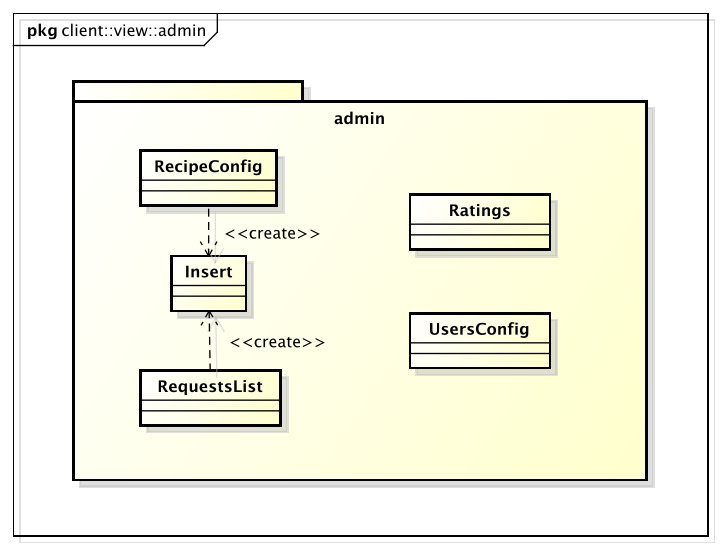
\includegraphics[scale=0.5]{./images/client/client_view_admin.pdf}}
	\caption{Package - client::view::admin}
\end{figure}

\begin{itemize}
	\item \textbf{Descrizione}: è il package che contiene tutte le pagine HTML che ha a disposizione l'utente che ha i privilegi di amministratore;\newline
	Per semplicità e chiarezza non è stato evidenziato nel grafico il fatto che ogni classe di questo package possiede un'istanza di MenuMain e di MenuSecondAdmin.
	\item \textbf{Padre}: client::view
	\item \textbf{Interazione con altri componenti}:
		\begin{itemize}
			\item client::controller::admin
		\end{itemize}
\end{itemize}

	\paragraph{Classi} % (fold)
		\subparagraph{client::view::admin::RecipeConfig} % (fold)
		\label{subp:bdsm_app_client_view_admin_recipeconfig}
			\begin{itemize}
				\item \textbf{Descrizione}: la classe rappresenta un template HTML per la visualizzazione dell'interfaccia di gestione delle Recipe;
				\item \textbf{Utilizzo}: viene utilizzata per generare la pagina HTML della gestione delle Recipe;
				\item \textbf{Relazioni con altre classi}:
					\begin{itemize}
						\item client::view::user::MenuMain
						\item client::view::admin::MenuSecondAdmin
						\item client::view::admin::Insert
						\item client::controller::admin::RecipeConfigRoute
						\item client::controller::admin::RecipeConfigCtrl
					\end{itemize}
			\end{itemize}
		% subparagraph bdsm_app_client_view_admin_recipeconfig (end)

		\subparagraph{client::view::admin::RequestList} % (fold)
		\label{subp:bdsm_app_client_view_admin_requestlist}
			\begin{itemize}
				\item \textbf{Descrizione}: la classe rappresenta un template HTML per la visualizzazione della pagina di visione delle richieste di Recipe;
				\item \textbf{Utilizzo}: viene utilizzata per generare la pagina HTML della lista delle richieste di Recipe;
				\item \textbf{Relazioni con altre classi}:
					\begin{itemize}
						\item client::view::user::MenuMain
						\item client::view::admin::MenuSecondAdmin
						\item client::view::admin::Insert
						\item client::controller::admin::RequestListRoute
						\item client::controller::admin::RequestListCtrl
					\end{itemize}
			\end{itemize}
		% subparagraph bdsm_app_client_view_admin_requestlist (end)

		\subparagraph{client::view::admin::Insert} % (fold)
		\label{subp:bdsm_app_client_view_admin_insert}
			\begin{itemize}
				\item \textbf{Descrizione}: la classe rappresenta un template HTML per la visualizzazione dell'interfaccia di inserimento di una nuova Recipe;
				\item \textbf{Utilizzo}: viene utilizzata per generare la pagina HTML di inserimento di una nuova recipe;
				\item \textbf{Relazioni con altre classi}:
					\begin{itemize}
						\item client::view::user::MenuMain
						\item client::view::admin::MenuSecondAdmin
						\item client::view::admin::RecipeConfig
						\item client::view::admin::RequestList
						\item client::controller::admin::RecipeConfigRoute
						\item client::controller::admin::InsertRecipeCtrl
					\end{itemize}
			\end{itemize}
		% subparagraph bdsm_app_client_view_admin_insert (end)

		\subparagraph{client::view::admin::Ratings} % (fold)
		\label{subp:bdsm_app_client_view_admin_ratings}
			\begin{itemize}
				\item \textbf{Descrizione}: la classe rappresenta un template HTML per la visualizzazione della pagina dei voti assegnati alle varie Recipe;
				\item \textbf{Utilizzo}: viene utilizzata per generare la pagina HTML di visione dei voti delle Recipe;
				\item \textbf{Relazioni con altre classi}:
					\begin{itemize}
						\item client::view::user::MenuMain
						\item client::view::admin::MenuSecondAdmin
						\item client::controller::admin::RatingsRoute
						\item client::controller::admin::RatingsCtrl
					\end{itemize}
			\end{itemize}
		% subparagraph bdsm_app_client_view_admin_ratings (end)

		\subparagraph{client::view::admin::UsersConfig} % (fold)
		\label{subp:bdsm_app_client_view_admin_usersconfig}
			\begin{itemize}
				\item \textbf{Descrizione}: la classe rappresenta un template HTML per la visualizzazione dell'interfaccia di gestione degli utenti;
				\item \textbf{Utilizzo}: viene utilizzata per generare la pagina HTML di gestione degli utenti;
				\item \textbf{Relazioni con altre classi}:
					\begin{itemize}
						\item client::view::user::MenuMain
						\item client::view::admin::MenuSecondAdmin
						\item client::controller::admin::UsersConfigRoute
						\item client::controller::admin::UsersConfigCtrl
					\end{itemize}
			\end{itemize}
		% subparagraph bdsm_app_client_view_admin_usersconfig (end)

		\subparagraph{client::view::admin::MenuSecondAdmin} % (fold)
		\label{subp:bdsm_app_client_view_admin_menusecondadmin}
			\begin{itemize}
				\item \textbf{Descrizione}: la classe rappresenta un template HTML per la creazione del menù secondario di un utente amministratore;
				\item \textbf{Utilizzo}: viene usata nel generare ogni pagina di un utente autenticato amministratore per generare il menù secondario;
				\item \textbf{Classi ereditate}:
					\begin{itemize}
						\item client::view::user::Menu
						\item client::view::user::MenuSecond
					\end{itemize}
				\item \textbf{Relazioni con altre classi}:
					\begin{itemize}
						\item client::view::user::Menu
						\item client::view::user::MenuSecond
						\item client::controller::admin::MenuSecondAdminCtrl
					\end{itemize}
			\end{itemize}
		% subparagraph bdsm_app_client_view_admin_menusecondadmin (end)

% subsubsection bdsm_app_client_view_admin (end)
